\section{TINJAUAN PUSTAKA}

% Ubah konten-konten berikut sesuai dengan isi dari tinjauan pustaka
\subsection{Hasil penelitian/perancangan terdahulu}
\subsubsection{Kendali mobil robot menggunakan isyarat tangan berbasis arduino}
Pada November 2020, Jati Widyo Leksono, Agung Samudra, Nanndo Yannuansa, dan Ahmad Fauzi membuat jurnal mengenai sistem kendali mobil robot menggunakan isyarat tangan. Dalam penelitian ini akan dilakukan pengembangan mobil robot yang mampu berjalan sesuai dengan isyarat tangan atau gestur tangan yang diberikan oleh user. Pada telapak tangan user nantinya akan ditempelkan suatu sensor yang mampu membaca pergerakan telapak tangan menurun, naik, kiri, kanan, dan mendatar. Dari pembacaan sensor tersebut data akan dikirimkan menuju receiver yang terdapat pada robot secara wireless \parencite{JurnalElectroLuecat}.

\subsection{Teori Dasar}
\subsubsection{Estimasi Pose tangan}
Pose tangan adalah potongan-potongan dari gerakan tangan yang betujuan untuk mengirimkan sinyal visual kepada penerima. Setiap pose dapat memiliki arti tersendiri sesuai dengan kesepakatan umum ataupun personal yang melakukan komunikasi \parencite{gesturtangan}. Pengenalan gestur atau pose tangan merupakan topik yang menarik dalam ilmu komputer dan teknologi yang betujuan untuk komunikasi antara manusia dengan komputer menggunakan gestur tanpa menyentuhnya secara langsung. Saat ini banyak \textit{framework} atau \textit{library} pembelajaran mesinuntuk mengenali gerakan tangan, salah satu yaitu Mediapipe. Mediapipe merupakan suatu framework yang dirancang oleh Google untuk menghasilkan audio atau video dari membangun \textit{pipelines} untuk mengolah data persepsi. Dengan bantuan dari Mediapipe tangan yang terdapat pada citra akan dapat dideteksi. Proses pertama yaitu akan mendeteksi telapak tangan atau disebut \textit{palm detection} agar program dapat mendeteksi keberadaan tangan. Selanjutnya yaitu mendeteksi 21 titik \textit{keypoint} dalam tangan yang sudah terdeteksi \parencite{UniversitasDinamika}. 

\begin{figure}[!h]
  \centering
	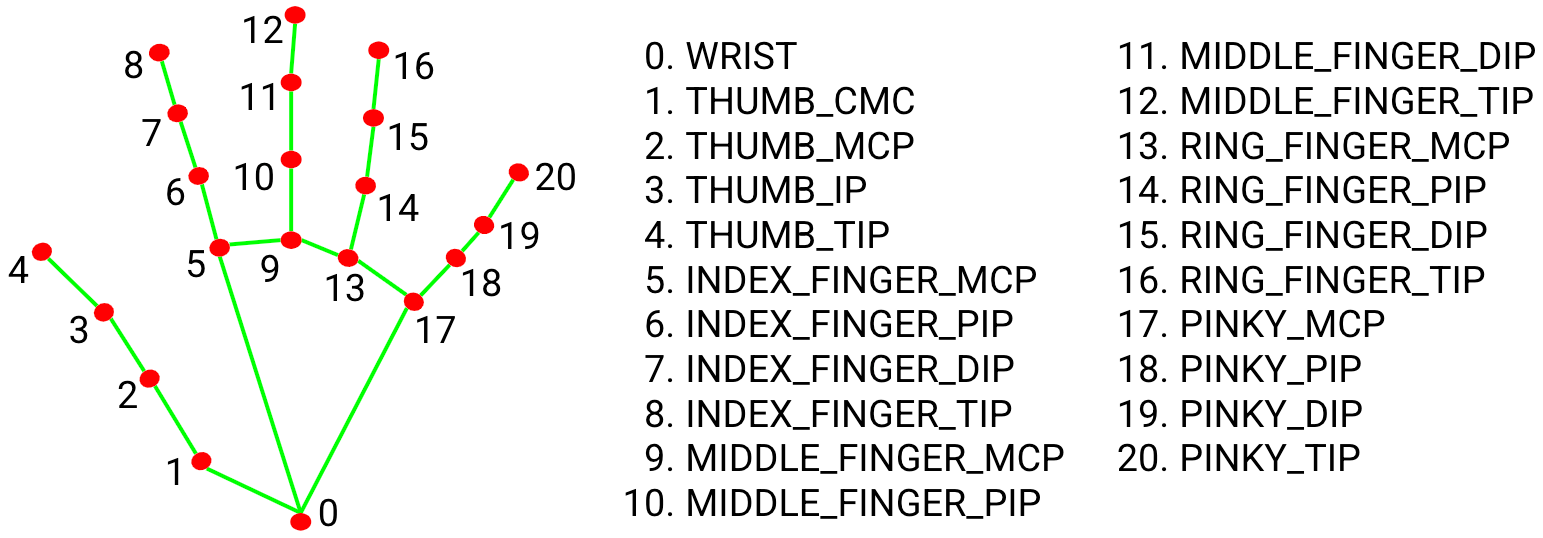
\includegraphics[width=1\linewidth]{gambar/hand_landmarks.png}
	\caption{21 titik \textit{keypoint} pada tangan \parencite{mediapipe}}
	\label{fig:tangan}
\end{figure}

\subsubsection{\textit{Convolutional Neural Network} (CNN)}
\textit{Convolutional Neural Network} atau biasa dikenal CNN merupakan salah satu dari \textit{neural network} yang digunakan untuk memproses data berupa grid. Salah satu contoh dari data grid adalah citra. Citra dianggap sebagai grid karena berbentuk piksel 2 dimensi. CNN dianggap sebagai salah satu solusi untuk permasalahan pada bidang \textit{Computer Vision} untuk mendeteksi dan mengenali sebuah image \parencite{CNN}. Secara nama \textit{Convolutional Neural Network} menunjukkan bahwa operasi matematika yang akan digunakan yaitu konvolusi dengan cara mengkalikan data 2 dimensi dengan kernel. Pada CNN akan memiliki 3 lapisan utama yaitu :
\begin{enumerate}
  \item \textit{Convolutional layer} \\
  Layer ini merupakan inti dari CNN karena pada layer ini akan dilakukannya operasi konvolusi. Operasi konvolusi pada layer ini akan dilakukan antara input data dengan \textit{filter} atau \textit{kernel}. \textit{Filter} akan melintasi input data dan akan melakukan operasi "dot" antara input data dengan nilai dari \textit{filter} sehingga akan menghasilkan \textit{feature map} \parencite{LinaQ}.
  
  \item \textit{Pooling layer} \\
  Layer ini digunakan untuk melakukan \textit{downsampling} yang berguna untuk mengurangi dimensi dan jumlah parameter. Terdapat 2 jenis \textit{pooling} yang sering digunakan yaitu \textit{max pooling} dan  \textit{average pooling}. \textit{Max pooling} adalah mengambil citra maksimum yang dicakup oleh kernel, sedangkan pada \textit{average pooling} adalah mengambil nilai rata-rata dari citra yang dicakup kernel.
  Namun tidak hanya itu \textit{pooling layer} juga digunakan untuk mengekstraksi fitur dominan \Parencite{Bukusakti}. 

  \item \textit{Fully connected layer} \\
  Layer ini digunakan untuk melakukan transformasi pada dimensi data agar dapat diklasifikasikan secara liner.
  Hasil dari \textit{pooling layer} masih berbentuk \textit{multidimensional array}, maka dari itu pada \textit{fully connected layer} akan dilakukan \textit{reshape} input dari \textit{multidimensional array} menjadi vector. Setiap \textit{neuron} pada \textit{convolutional layer} akan ditransformasikan menjadi data satu dimensi sebelum dapat dimasukkan dalam sebuah \textit{fully connected layer} \parencite{JurnalTeknikITS}.

  \begin{figure}[!h]
    \centering
    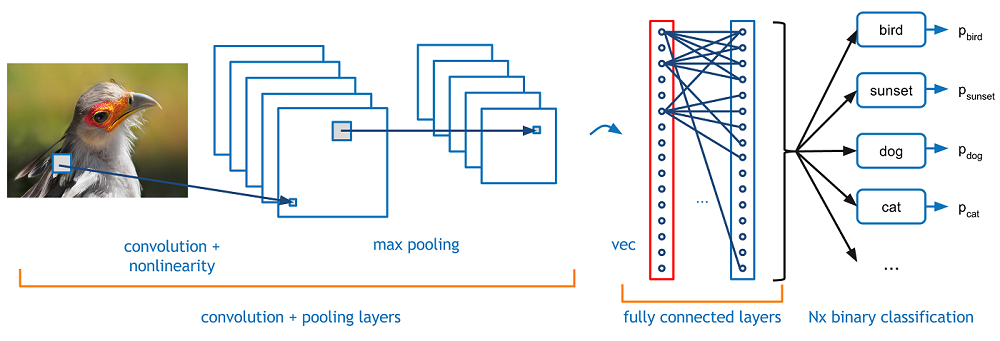
\includegraphics[width=1\linewidth]{gambar/cnn.png}
    \caption{Arsitektur CNN \parencite{adit}}
    \label{fig:cnn}
  \end{figure}

\end{enumerate} 

